\documentclass[12pt, a4paper, onecolumn, answers]{exam}

\usepackage[top = 1 in, bottom = 1 in, left = 0.8 in, right = 0.8 in]{geometry}

\usepackage{amsmath}
\allowdisplaybreaks[1]
\usepackage{amssymb, amsfonts}
\usepackage{enumerate}
\usepackage{multirow}
\usepackage{hhline}
\usepackage{array}
\usepackage{booktabs}
\usepackage{longtable}
\usepackage{graphicx}
\usepackage{tabularx}
\usepackage{tabularray}
\usepackage{undertilde}
\usepackage{dingbat}
\usepackage{fontawesome5}
\usepackage{tasks}
\usepackage{bbding}
\usepackage{twemojis}
% how to use bull's eye ----- \scalebox{2.0}{\twemoji{bullseye}}
\usepackage{customdice}
% how to put dice face ------ \dice{2}
\usepackage{pgfplots}
\pgfplotsset{compat=1.17}


\begin{document}

\begingroup  
    \centering
    \LARGE MSMS-306 : Lifetime Data Analysis\\
    \LARGE Assignment : 01\\[0.5em]
    \large \today\\[0.5em]
    \large Ananda Biswas\par
    \large Exam Roll Number : 24419STC053 \par
    \large M.Sc. Statistics \& Computing (Semester - III)\par
\endgroup
\rule{\textwidth}{0.4pt}
\pointsdroppedatright   %Self-explanatory
\printanswers
\unframedsolutions
\renewcommand{\solutiontitle}{\noindent\textbf{Ans:}\enspace}   %Replace "Ans:" with starting keyword in solution box

\begin{questions}

    \question \textcolor{blue}{Question : }Establish the exponential distribution as a suitable lifetime model by analyzing its key characteristics with graphical illustrations. Also, compare it with other standard lifetime models, highlighting its advantages and limitations.
    
    
\begin{solution}
Lifetime data / survival time data measure the \underline{time to a certain event}, such as failure, death etc. These times are subject to random variations, and like any random variables, form a \underline{probability distribution}. \\[0.15em]

Time$(T)$ is a non-negative continuous $(T \geq 0)$ quantity and the exponential distribution also has similar properties. That makes \underline{Exponential Distribution} one of the simplest distributions to model lifetime data.

The distribution of survival times is usually characterized by 3 functions as follows :
\begin{itemize}
\item the Probability Density Function
\item the Survival Function
\item the Hazard Function
\end{itemize}

There is also the Cumulative Hazard Function.

\vspace{0.1cm}

\leftpointright \hspace{0.1cm} \underline{Probability Density Function} : If the lifetime $T$  follows the exponential distribution with \underline{rate $\lambda \in \mathbb{R^{+}}$}, the probability density function $f : (-\infty, \infty) \rightarrow [0, \infty)$ is given by

\begin{equation*}
	 f(t) =
		\begin{cases}
		 \lambda e^{-\lambda t}, & t > 0  \\
		 0, & \text{otherwise}.
		\end{cases}
\end{equation*}


\begin{minipage}{0.48\textwidth}
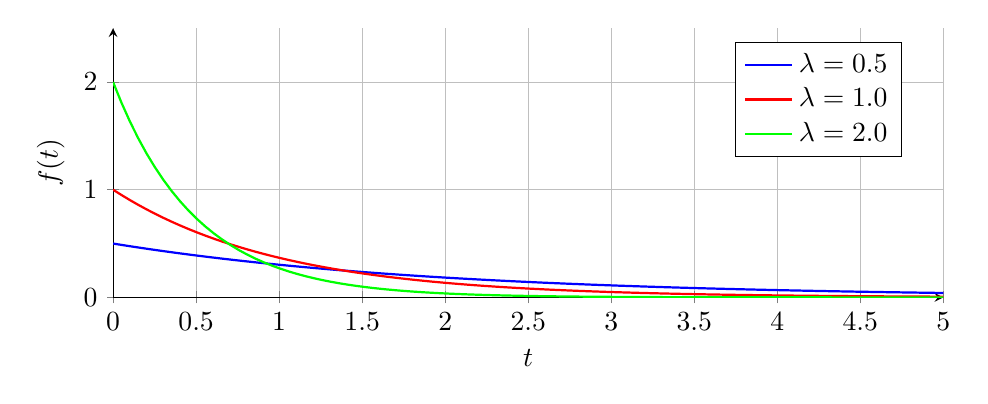
\begin{tikzpicture}
\begin{axis}[
    width=\textwidth,
    height=5cm,
    domain=0:5,
    samples=100,
    xlabel={$t$}, ylabel={$f(t)$},
    ymin=0, ymax=2.5,
    axis lines=left,
    grid=both,
    legend style={at={(0.95,0.95)}, anchor=north east},
]


    \addplot[blue, thick] {0.5*exp(-0.5*x)};
    \addlegendentry{$\lambda = 0.5$}



    \addplot[red, thick] {1.0*exp(-1.0*x)};
    \addlegendentry{$\lambda = 1.0$}


    \addplot[green, thick] {2.0*exp(-2.0*x)};
    \addlegendentry{$\lambda = 2.0$}


\end{axis}
\end{tikzpicture}
\end{minipage}
\hfill
\begin{minipage}{0.48\textwidth}
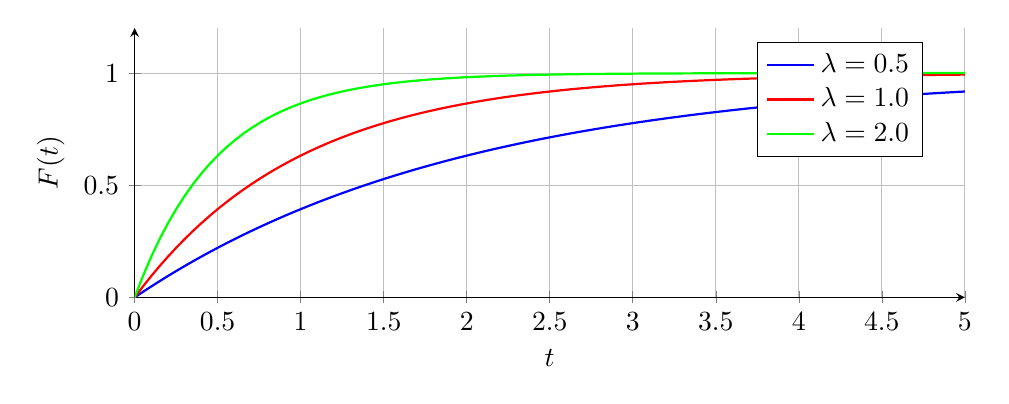
\begin{tikzpicture}
\begin{axis}[
    width=\textwidth,
    height=5cm,
    domain=0:5,
    samples=100,
    xlabel={$t$}, ylabel={$F(t)$},
    ymin=0, ymax=1.2,
    axis lines=left,
    grid=both,
    legend style={at={(0.95,0.95)}, anchor=north east},
]


    \addplot[blue, thick] {1-exp(-0.5*x)};
    \addlegendentry{$\lambda = 0.5$}



    \addplot[red, thick] {1-exp(-1.0*x)};
    \addlegendentry{$\lambda = 1.0$}


    \addplot[green, thick] {1-exp(-2.0*x)};
    \addlegendentry{$\lambda = 2.0$}


\end{axis}
\end{tikzpicture}
\end{minipage}


\leftpointright \hspace{0.1cm} \underline{Survival Function} : From definition, with $F(\cdot)$ being the CDF of $T$, Survival function $S : [0, \infty) \rightarrow [0, 1]$ is given by $$S(t) = P[T > t] = 1 - F(t) \,\, \forall t \geq 0.$$

We calculate

\begin{align*}
\forall t \geq 0, \,\, F(t) &= \int \limits_{0}^{t} f(x) dx \\
&= \int \limits_{0}^{t} \lambda e^{-\lambda x} dx = \lambda \left[-\dfrac{e^{-\lambda x}}{\lambda}\right]_{0}^{t} \\
&= 1 - e^{-\lambda t}
\end{align*}

\therefore \hspace{0.1cm} $S(t) = e^{-\lambda t} \,\, \forall t \geq 0$

\begin{center}
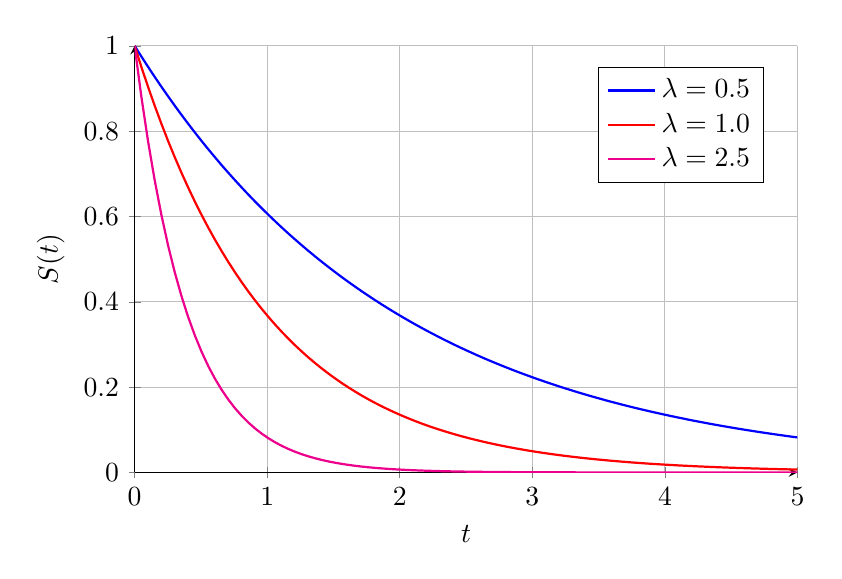
\begin{tikzpicture}
 \begin{axis}[
    width=10cm,
    height=7cm,
    domain=0:5,
    samples=100,
    xlabel={$t$},
    ylabel={$S(t)$},
    ymin=0, ymax=1,
    axis lines=left,
    grid=both,
    legend style={at={(0.95,0.95)}, anchor=north east}
]


    \addplot[blue, thick] {exp(-0.5*x)};
    \addlegendentry{$\lambda = 0.5$}

    \addplot[red, thick] {exp(-1.0*x)};
    \addlegendentry{$\lambda = 1.0$}

    \addplot[magenta, thick] {exp(-2.5*x)};
    \addlegendentry{$\lambda = 2.5$}

\end{axis}
\end{tikzpicture}
\end{center}

\leftpointright \hspace{0.1cm} \underline{Hazard Function} : The Hazard function $h : [0, \infty) \rightarrow [0, \infty)$ is defined as
\[
h(t) = \lim \limits_{\Delta t \to 0} \dfrac{
   P\left[
    \begin{array}{c}
      \text{an individual fails in the time interval } (t, t + \Delta t) \\
      \text{given the individual has survived to } t
    \end{array}
  \right]
}{
  \Delta t
}
\,\, \forall t \geq 0.
\]

A simple derivation leads to $$h(t) = \dfrac{f(t)}{S(t)} \,\, \forall t \geq 0.$$

Here we have
\begin{itemize}
\item $f(t) = \lambda e^{-\lambda t} \cdot I_{(0, \infty)}(t), \,\, \lambda > 0$.
\item $S(t) = e^{-\lambda t} \,\, \forall t \geq 0$.
\end{itemize}

\vspace{0.5cm}

\therefore \hspace{0.1cm} $h(t) = \lambda \,\, \forall t \geq 0$, a constant, independent of $t$.

\vspace{0.5cm}

\smallpencil \hspace{0.1cm} A constant hazard rate is a \underline{necessary and sufficient} condition for a continuous lifetime distribution to be exponential.

\begin{center}
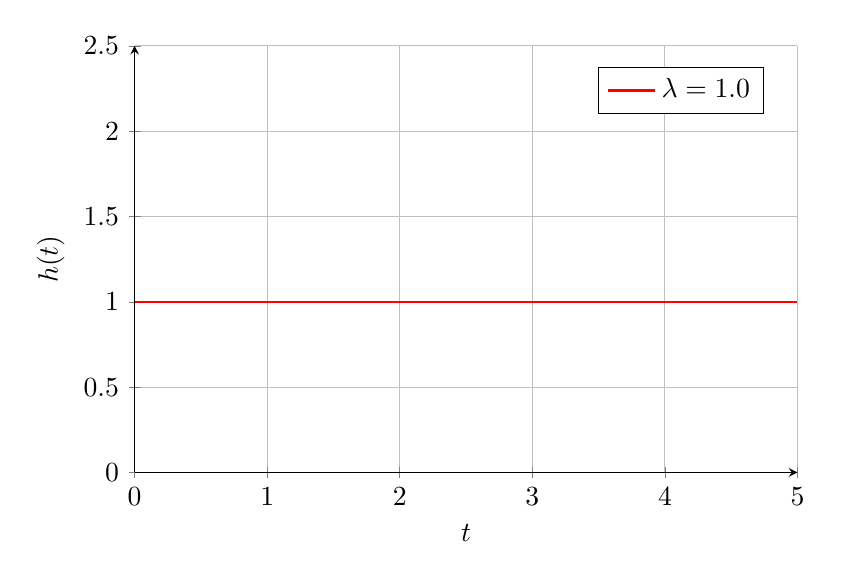
\begin{tikzpicture}
 \begin{axis}[
    width=10cm,
    height=7cm,
    domain=0:5,
    samples=100,
    xlabel={$t$},
    ylabel={$h(t)$},
    ymin=0, ymax=2.5,
    axis lines=left,
    grid=both,
    legend style={at={(0.95,0.95)}, anchor=north east}
]


    \addplot[red, thick] {1.0};
    \addlegendentry{$\lambda = 1.0$}

\end{axis}
\end{tikzpicture}
\end{center}

\leftpointright \hspace{0.1cm} \underline{Cumulative Hazard Function} : The Cumulative Hazard Function $H : [0, \infty) \rightarrow [0, \infty)$ is defined by $$H(t) = \int \limits_{0}^{t} h(x) dx.$$

For $T \sim \text{Exp}(\text{rate} = \lambda)$, $$H(t) = \lambda t \,\, \forall t \geq 0.$$

\begin{center}
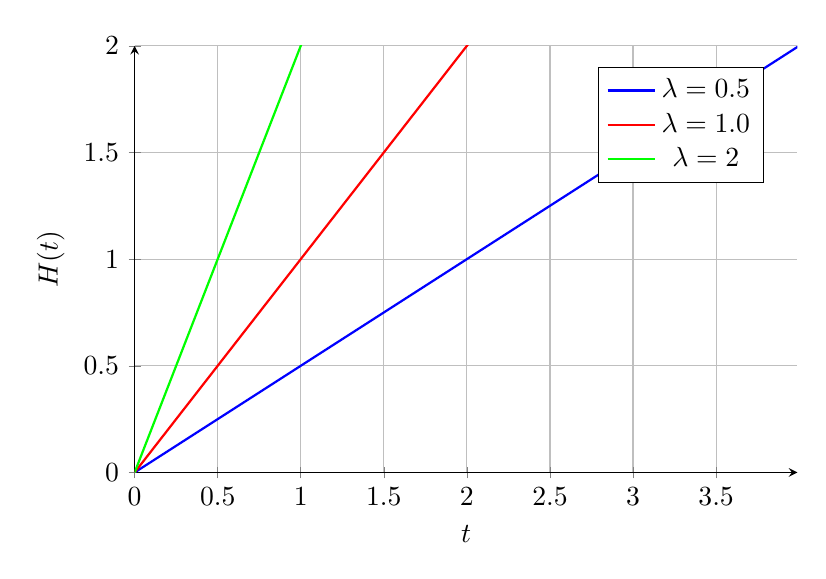
\begin{tikzpicture}
 \begin{axis}[
    width=10cm,
    height=7cm,
    domain=0:5,
    samples=100,
    xlabel={$t$},
    ylabel={$H(t)$},
    ymin=0, ymax=2,
    axis lines=left,
    grid=both,
    legend style={at={(0.95,0.95)}, anchor=north east}
]

    \addplot[blue, thick] {0.5*x};
    \addlegendentry{$\lambda = 0.5$}

    \addplot[red, thick] {1.0*x};
    \addlegendentry{$\lambda = 1.0$}

    \addplot[green, thick] {2*x};
    \addlegendentry{$\lambda = 2$}

\end{axis}
\end{tikzpicture}
\end{center}

\end{solution}

\end{questions}

\newpage

\begin{center}
    \large \textbf{Comparison of Exponential Distribution with Other\\ Standard Lifetime Models}
\end{center}

\begin{table}[h!]
\def\arraystretch{1.5}
\centering
\begin{tabularx}{\textwidth}{>{\raggedright\arraybackslash}p{3.5cm} 
                              >{\raggedright\arraybackslash}p{2.5cm} 
                              >{\raggedright\arraybackslash}p{2.5cm}
                              >{\raggedright\arraybackslash}p{2.5cm} 
                              >{\raggedright\arraybackslash}p{2.5cm} 
                              >{\raggedright\arraybackslash}p{2.5cm}}
\toprule
\textbf{Basis of Distinction} & \textbf{Exponential} & \textbf{Weibull} & \textbf{Gamma} & \textbf{Lognormal} & \textbf{Pareto} \\
\midrule

\textbf{Hazard Function (Failure Rate)} 
& Constant over time (no change) 
& Can increase or decrease based on shape 
& Usually increases with time 
& Increases first, then decreases (hump-shaped) 
& Decreases as time increases \\

\textbf{Memoryless Property} 
& Yes
& No
& No
& No
& No \\

\textbf{Tail Behaviour (Extreme Events)} 
& Light tails — extreme values are rare 
& Light tails — few extreme values 
& Moderate tails — some large values possible 
& Heavy tails — large values more common 
& Very heavy tails — high chance of extremes \\

\textbf{Real-life Use Cases} 
& Lifetimes of bulbs, radioactive decay 
& Mechanical systems, reliability engineering 
& Queues, survival analysis 
& Financial time durations, web session times 
& Insurance, wealth, income distribution \\

\textbf{Mathematical Simplicity} 
& Easiest
& Moderate
& Slightly complex
& Complex
& Moderate \\

\bottomrule
\end{tabularx}
\caption{Comparison of exponential distribution with other standard lifetime models}
\end{table}



\newpage


\subsection*{Advantages of Exponential Distribution}

\begin{longtable}{@{}p{4cm}p{11cm}@{}}
\toprule
\textbf{Compared With} & \textbf{Advantage of Exponential Distribution} \\ \midrule
\textbf{Weibull} & Simpler to use and interpret. It has only one parameter (\(\lambda\)), making it easier to estimate. Suitable when the failure rate is constant over time. \\
\textbf{Gamma} & Computationally less intensive. Exponential is a special case of Gamma when shape = 1, so it works when only a single failure phase is present. \\
\textbf{Lognormal} & Easier to analyze mathematically. Exponential has memoryless property, unlike lognormal. Useful in simpler reliability models. \\
\textbf{Pareto} & Has lighter tails, making it better for modeling systems without extreme outliers. Also easier to fit and simulate. \\ 
\bottomrule
\end{longtable}

\vspace{1cm}

\subsection*{Limitations of Exponential Distribution}

\begin{longtable}{@{}p{4cm}p{11cm}@{}}
\toprule
\textbf{Compared With} & \textbf{Limitation of Exponential Distribution} \\ \midrule
\textbf{Weibull} & Assumes constant failure rate, which is unrealistic in many aging systems. Weibull can model increasing or decreasing failure rates. \\
\textbf{Gamma} & Can't model multi-stage failure processes. Gamma handles systems that degrade over multiple phases more effectively. \\
\textbf{Lognormal} & Cannot model “typical” failure times with a peak. Lognormal captures bell-shaped distributions of lifetimes. \\
\textbf{Pareto} & Doesn’t model rare/extreme events well. Pareto has heavy tails, useful for risk modeling and extreme lifetimes. \\
\bottomrule
\end{longtable}


\end{document}